\documentclass[times, twoside]{zHenriquesLab-StyleBioRxiv}
\usepackage{blindtext}
\usepackage[utf8]{inputenc}
\usepackage{graphicx}

\DeclareMathOperator*{\E}{\mathbb{E}}
\newcommand{\norm}[1]{\left\lVert #1 \right\rVert}

% Please give the surname of the lead author for the running footer
\leadauthor{Denovellis} 

\begin{document}

\title{A state space model for discovering the trajectory dynamics of replay}
\shorttitle{Replay Dynamics}

% Use letters for affiliations, numbers to show equal authorship (if applicable) and to indicate the corresponding author
\author[4]{Eric L. Denovellis}
\author[2, 3]{Anna K. Gillespie}
\author[2, 3]{Michael E. Coulter}
\author[1]{Uri T. Eden}
\author[2, 3, 4, \Letter]{Loren M. Frank}


\affil[1]{Department of Mathematics and Statistics, Boston University, Boston, Massachusetts}
\affil[2]{Department of Physiology, University of California, San Francisco, San Francisco, California}
\affil[3]{Kavli Institute for Fundamental Neuroscience, University of California, San Francisco, San Francisco, California}
\affil[4]{Howard Hughes Medical Institute, University of California, San Francisco, San Francisco, California}

\maketitle

%TC:break Abstract
%the command above serves to have a word count for the abstract
\begin{abstract}
During sleep and immobility, hippocampal place cells fire in sequences consistent with temporally compressed versions of trajectories previously run by the animal. These replayed sequences are hypothesized to be an important mechanism for the retrieval of spatial memory in service of consolidation and decision-making. Replay events are typically evaluated based on whether they activate sequences of place cells that represent spatially continuous trajectories through the environment, but recent work has shown that these events can have more complex dynamics. For example, sequences can alternate between hovering on a particular spatial location and continuous movement or can represent continuous trajectories in other spatial environments, which may appear spatially incoherent in the context of the current environment.

To quantify the structure of replay events, we develop a state space model that uses a combination of discrete and continuous latent state to decompose place cell sequences into categories based on their latent dynamics. Each discrete latent “category” is associated with a type of continuous latent dynamic—hovering in place, spatially fragmented or spatially continuous. This allows for (1) direct comparison between different categories of sequence dynamics, (2) expression of our confidence in one or more categories explaining the data, and (3) characterization of the transitions between categories. In addition, the model can function in 2D, avoiding linearization errors on more complicated environments. We demonstrate the utility of this model on simulated and real data of an animal performing a spatial memory task.

\end {abstract}
%TC:break main
%the command above serves to have a word count for the abstract

\begin{keywords}
Hippocampus | Replay | State Space
\end{keywords}

\begin{corrauthor}
%\texttt{loren{@}phy.ucsf.edu}
loren\at phy.ucsf.edu
\end{corrauthor}

\section*{Introduction}
The hippocampus is a brain area that is important for short term learning and memory. Neurons in the hippocampus preferentially fire in response to specific locations in an environment, which results in sequences of cells firing as an animal moves through an environment that reflect the trajectory of the animal. When the animal is asleep or immobile, cells also fire in sequence, forming trajectory-like representations that can recapitulate sequences previously observed when the animal was running. These sequences are thought to be important for memory consolidation or prospective decision making. (cite some examples). Therefore, characterizing the dynamics of hippocampal sequences is important for understanding memory consolidation and prospective decision making.

Current methods analyze hippocampal sequences by assuming a constant velocity trajectory \cite{DavidsonHippocampalReplayExtended2009}, corresponding to a single dynamic. This is done by computing the probability of position at each time using the place field information from the population of neurons and then fitting a line to maximize the probability of position over time. If the probabilities near the best fit line are high relative to shuffled distribution, the replay is analyzed. Often, trajectories that travel less than a certain distance \cite{PfeifferAutoassociativedynamicsgeneration2015} are excluded.

However, there is a growing evidence that trajectories that have more complex dynamics. Farooq and Dragoi \cite{FarooqEmergencepreconfiguredplastic2019} found that juvenile rats . For example, Pfeiffer and Foster \cite{PfeifferAutoassociativedynamicsgeneration2015} found that trajectories alternated between stationary hovering trajectories and continuous movement trajectories on a gamma timescale. 

Our mathematical model precisely specifies the dyna

\section*{Results}

\begin{figure*}%[tbhp]
\centering
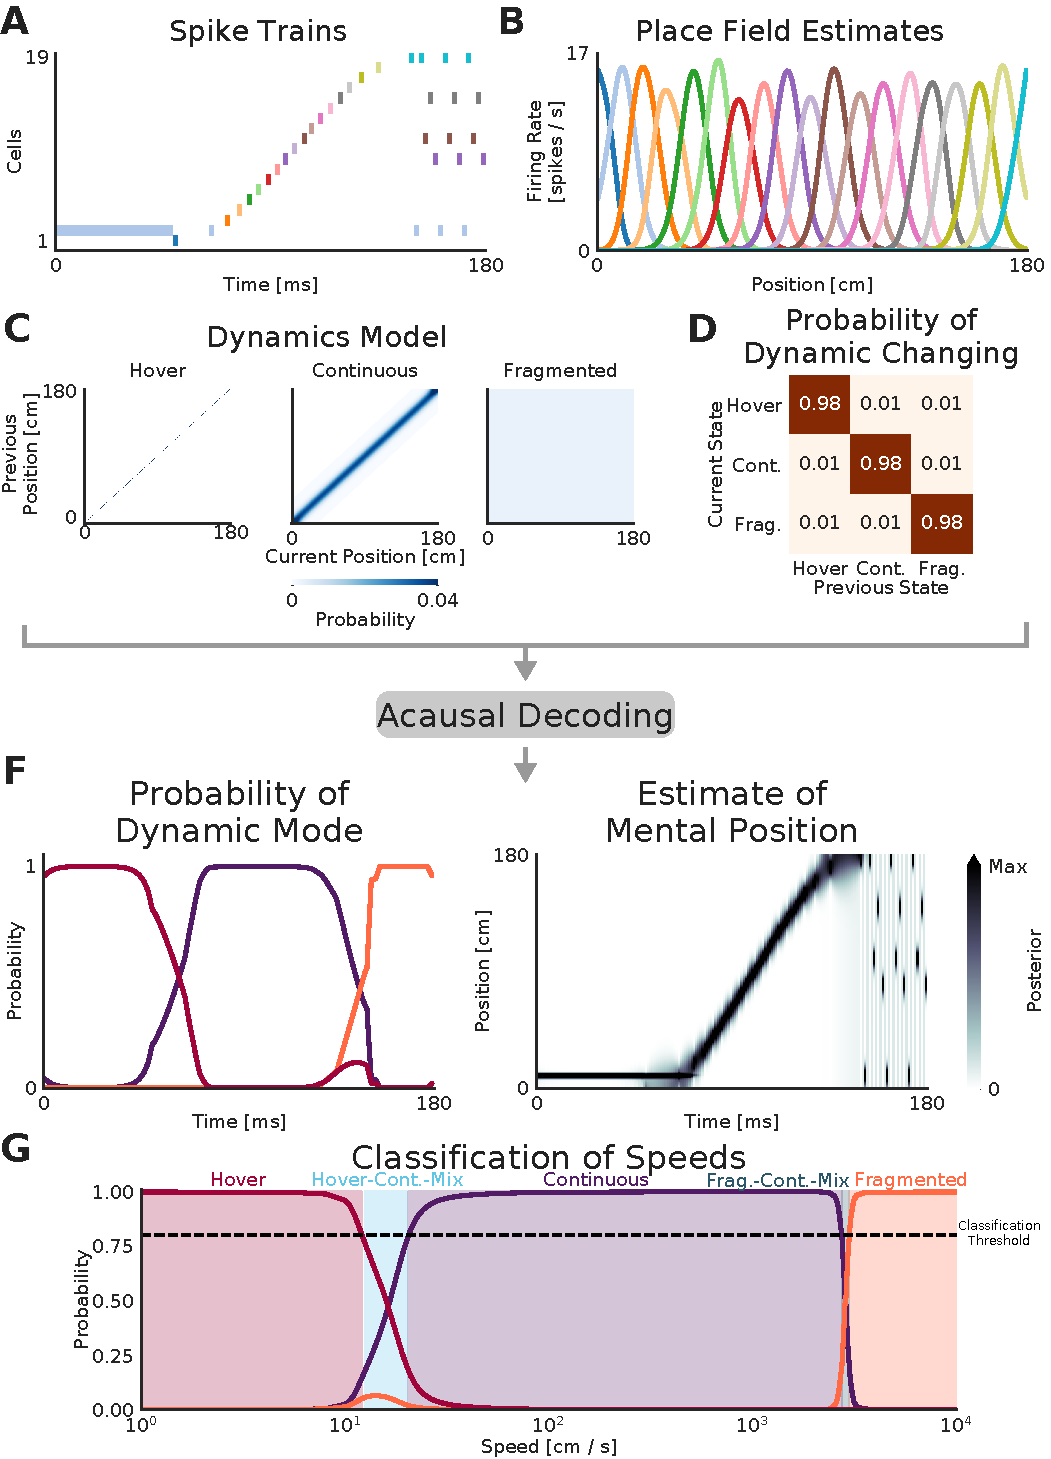
\includegraphics[width=0.80\linewidth]{figures/Figure1/Figure1_v3}
\caption{Placeholder image of Iris with a long example caption to show justification setting.}
\label{Figure1}
\end{figure*}

\begin{figure*}%[tbhp]
\centering
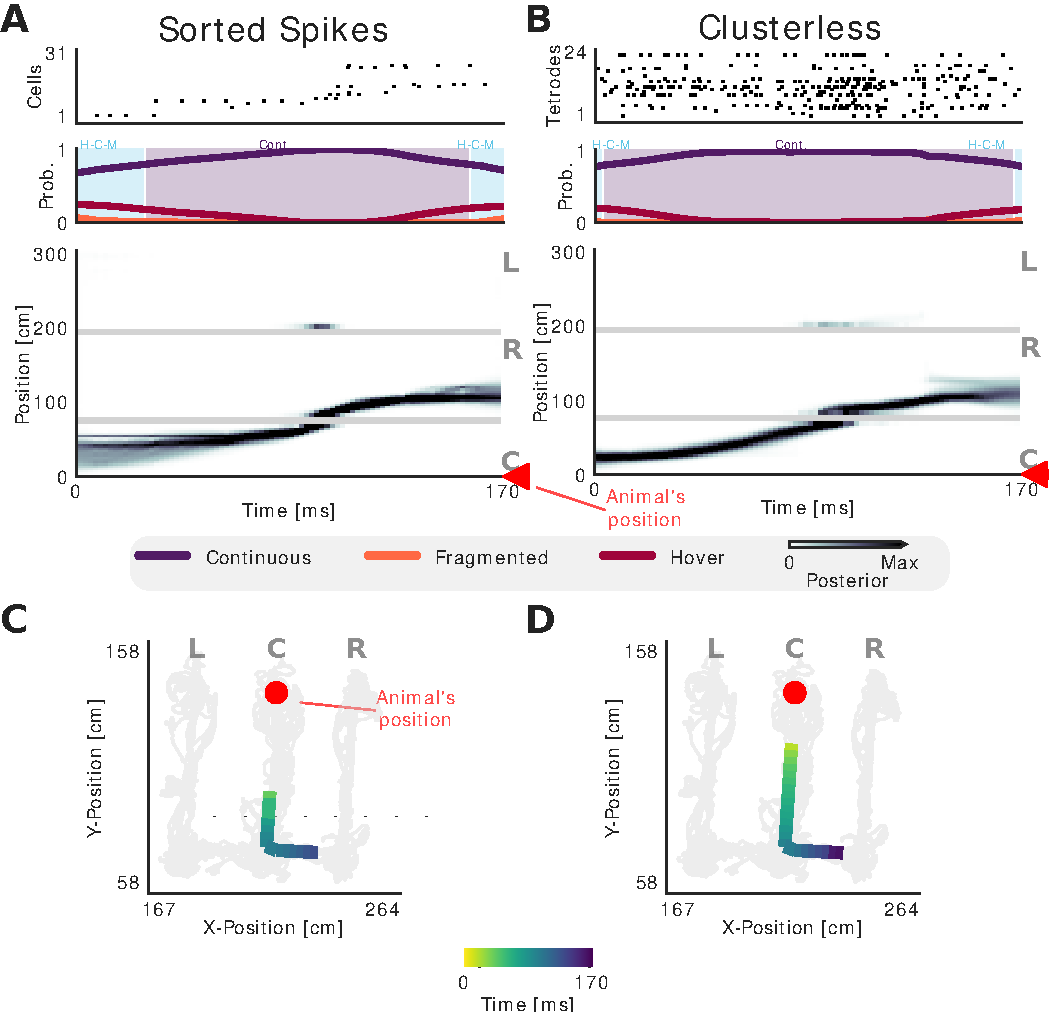
\includegraphics[width=0.80\linewidth]{figures/Figure2/Figure2_v3}
\caption{Placeholder image of Iris with a long example caption to show justification setting.}
\label{Figure2}
\end{figure*}

\begin{figure*}%[tbhp]
\centering
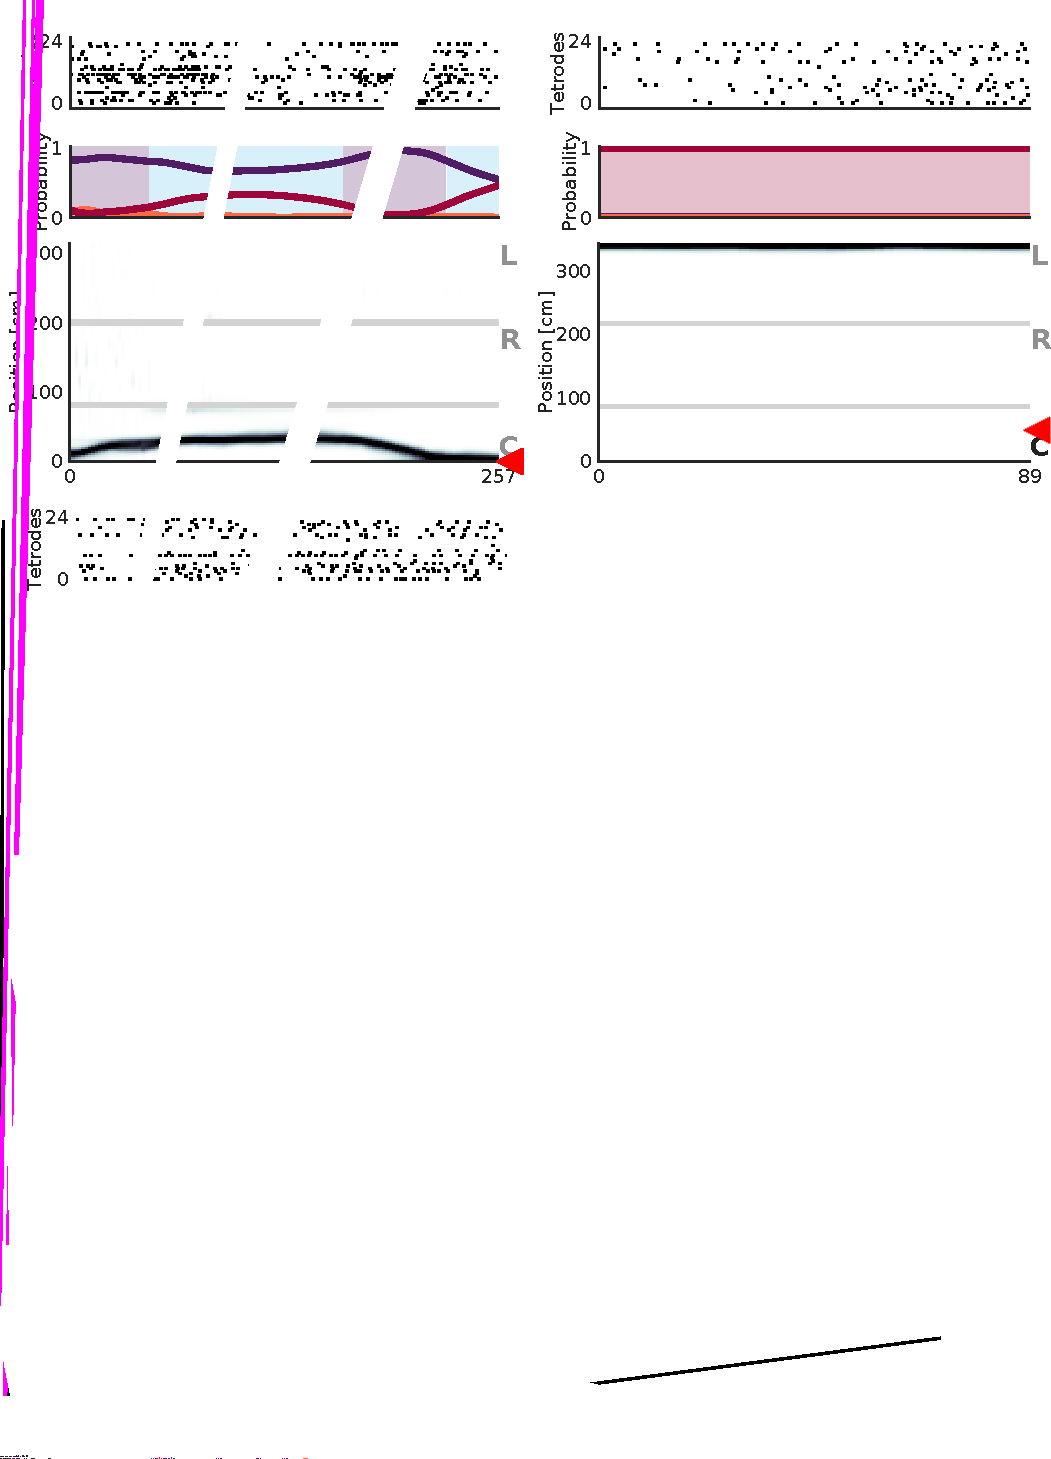
\includegraphics[width=0.80\linewidth]{figures/Figure3/Figure3_v3}
\caption{Placeholder image of Iris with a long example caption to show justification setting.}
\label{Figure3}
\end{figure*}

\begin{figure*}%[tbhp]
\centering
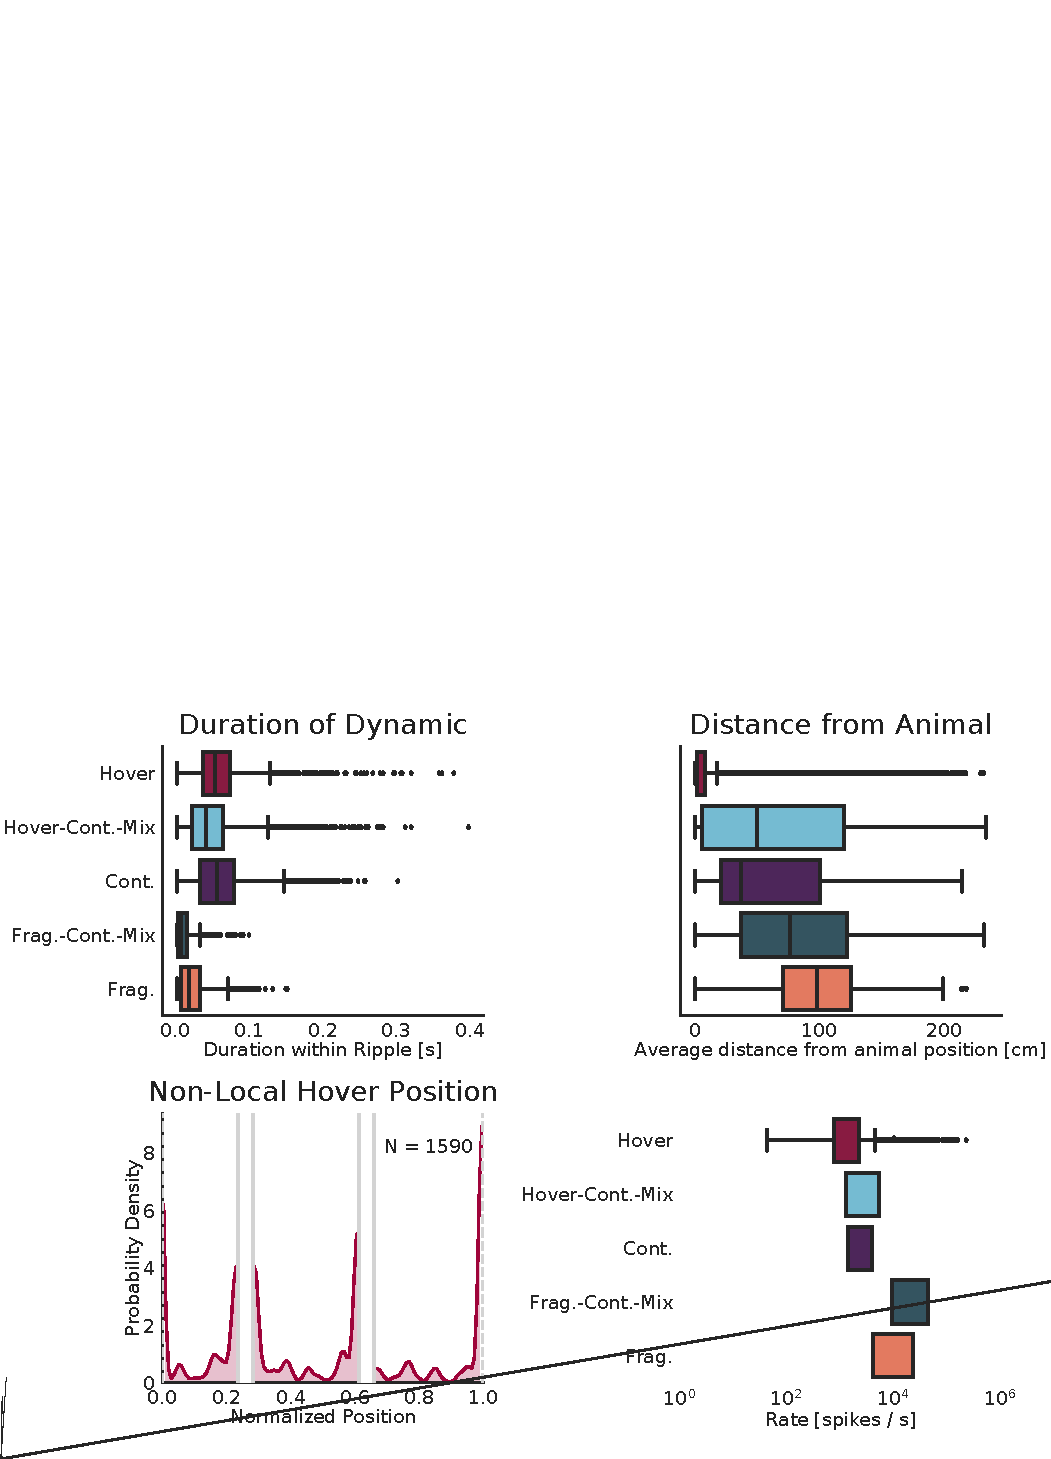
\includegraphics[width=0.80\linewidth]{figures/Figure4/Figure4_v2}
\caption{Placeholder image of Iris with a long example caption to show justification setting.}
\label{Figure4}
\end{figure*}


\section*{Discussion}


\subsection*{Blabla} 

\begin{acknowledgements}
\end{acknowledgements}

\section*{References}
\bibliography{refs}

\onecolumn
\newpage

\section*{Methods}
\subsection*{The Model}
The 

\subsection*{Encoding - Clusterless}
In order to encode how each tetrode's unsorted spiking activity relates to position, we use a marked point process framework. For each multiunit spike during movement (defined as time periods when the running speed is greater than 4 cm/s), the associated waveform features (the marks) and position are recorded in a (n-spikes, n-features + n-position-dimensions) array. In our case, the waveform features correspond to the max amplitude observed on each tetrode wire at the time of the multiunit spike. This array is used as the training samples in a kernel density estimator during the decoding step.

\subsection*{Encoding - Sorted Spikes}
In order to encode how each cell's spiking activity relates to position (the place field), we fit a generalized linear model (GLM) with a Poisson response distribution to each cell's spiking activity during movement (defined as time periods when the running speed is greater than 4 cm/s). We estimate the parameters $\beta$, which consist of $\beta_{0}$, the average firing rate over time, and $\beta_{i}$, weights for third degree B-splines basis functions $f_{i}$ over position (or tensor products of the B-splines when position is two dimensional). B-spline basis functions are used because place field firing activity is assumed to vary smoothly over position and this prior knowledge can be exploited to reduce the total number of model parameters needed. Each basis function is spaced every 5 cm over the range of the position and zero constrained so that the change encoded by the parameters is relative to the baseline firing rate. We use a log link function to convert the linear combination of parameters to an instantaneous firing rate over time $\lambda(t)$ to ensure the rate is always positive. 

$$log(\lambda(t)) = \beta_{0} + \sum_{i} f_{i}(position)\beta_{i}$$

A small L2 penalization term $-\lambda\norm{\beta_{i}}_{2}^{2}$ used to prevent model fitting instability when spiking activity is very low. We set this to 0.5 for all cells. Fitting is done by maximizing the penalized likelihood using a Newton-Raphson algorithm.

\subsection*{Decoding - Clusterless}


\subsection*{Simulated Data}

\subsection*{Data}

\subsection*{Software and Code availability}
Python code used for analysis and generating figures in the paper is available at: \url{https://github.com/Eden-Kramer-Lab/replay_trajectory_paper}. Code for the classifier is available in a separate software repository to facilitate code reuse at: \url{https://github.com/Eden-Kramer-Lab/replay_trajectory_classification}. All code is open-source and licensed under the MIT Software License. Classifier code can be easily installed as a python package with all requisite dependencies using pip or conda. See software repositories for specific details.

\newpage

%%%%%%%%%%%%%%%%%%%%%%%%%%%%%
% Supplementary Information %
%%%%%%%%%%%%%%%%%%%%%%%%%%%%%
\captionsetup*{format=largeformat}

\begin{figure*}%[tbhp]
\centering
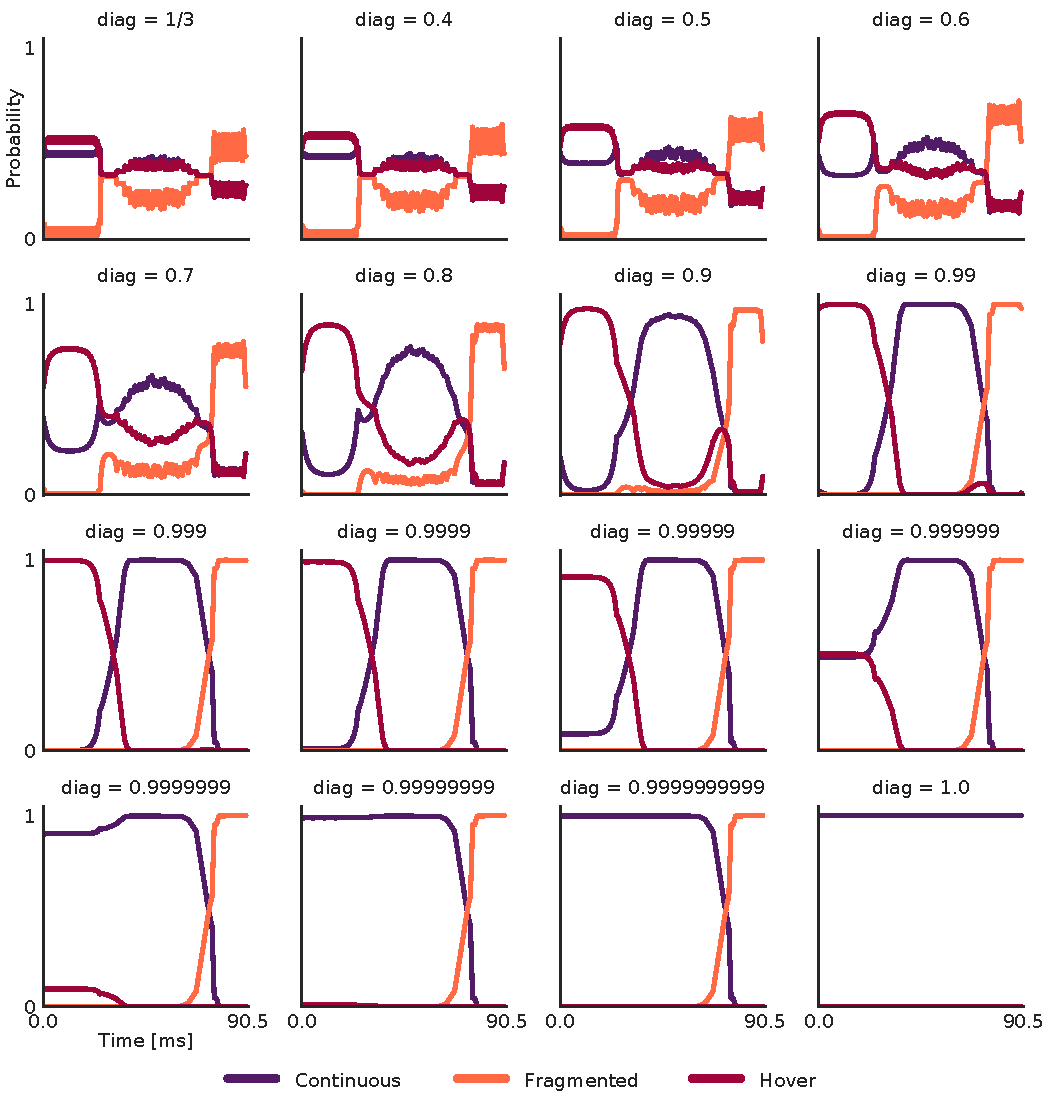
\includegraphics[width=0.80\linewidth]{figures/Figure1-supplemental1/Figure1_v1_supplemental1}
\caption{Placeholder image of Iris with a long example caption to show justification setting.}
\label{fig:Figure1-Figure supplement 1}
\end{figure*}

\begin{figure*}%[tbhp]
\centering
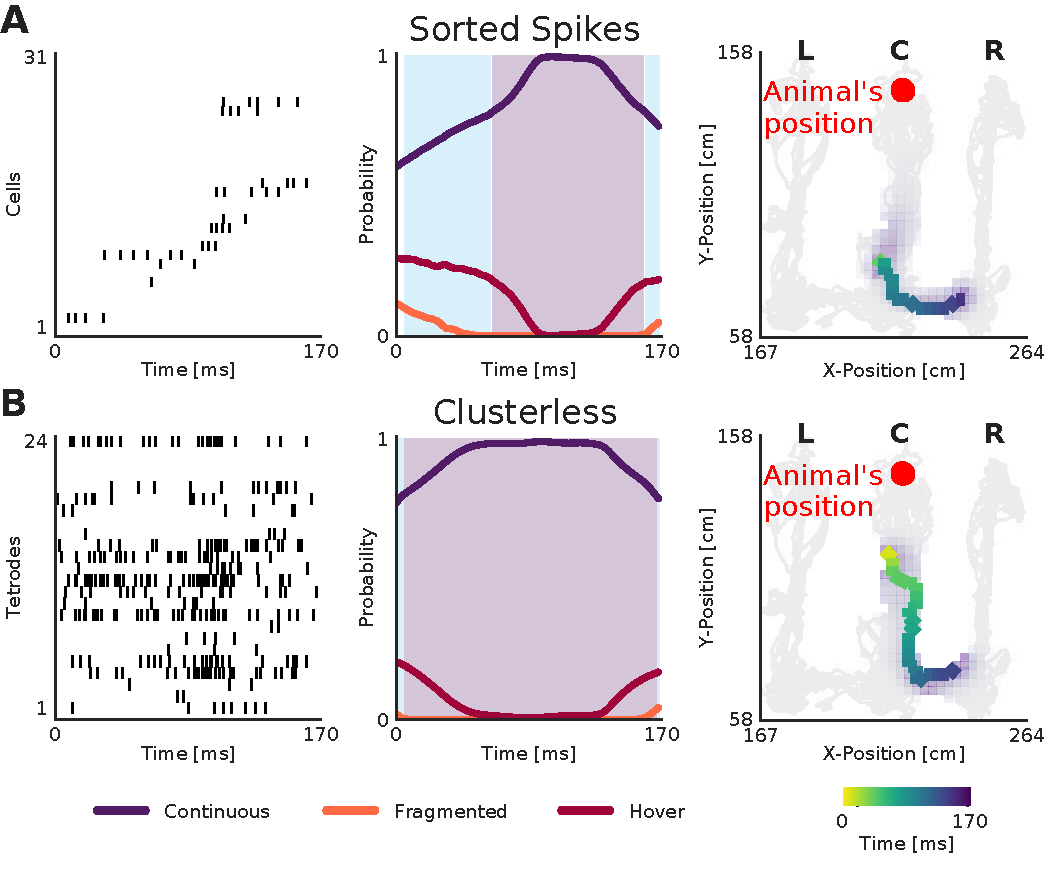
\includegraphics[width=0.80\linewidth]{figures/Figure2-supplemental1/Figure2_v2-supplemental1}
\caption{Placeholder image of Iris with a long example caption to show justification setting.}
\label{fig:Figure2-Figure supplement 1}
\end{figure*}

\begin{figure*}%[tbhp]
\centering
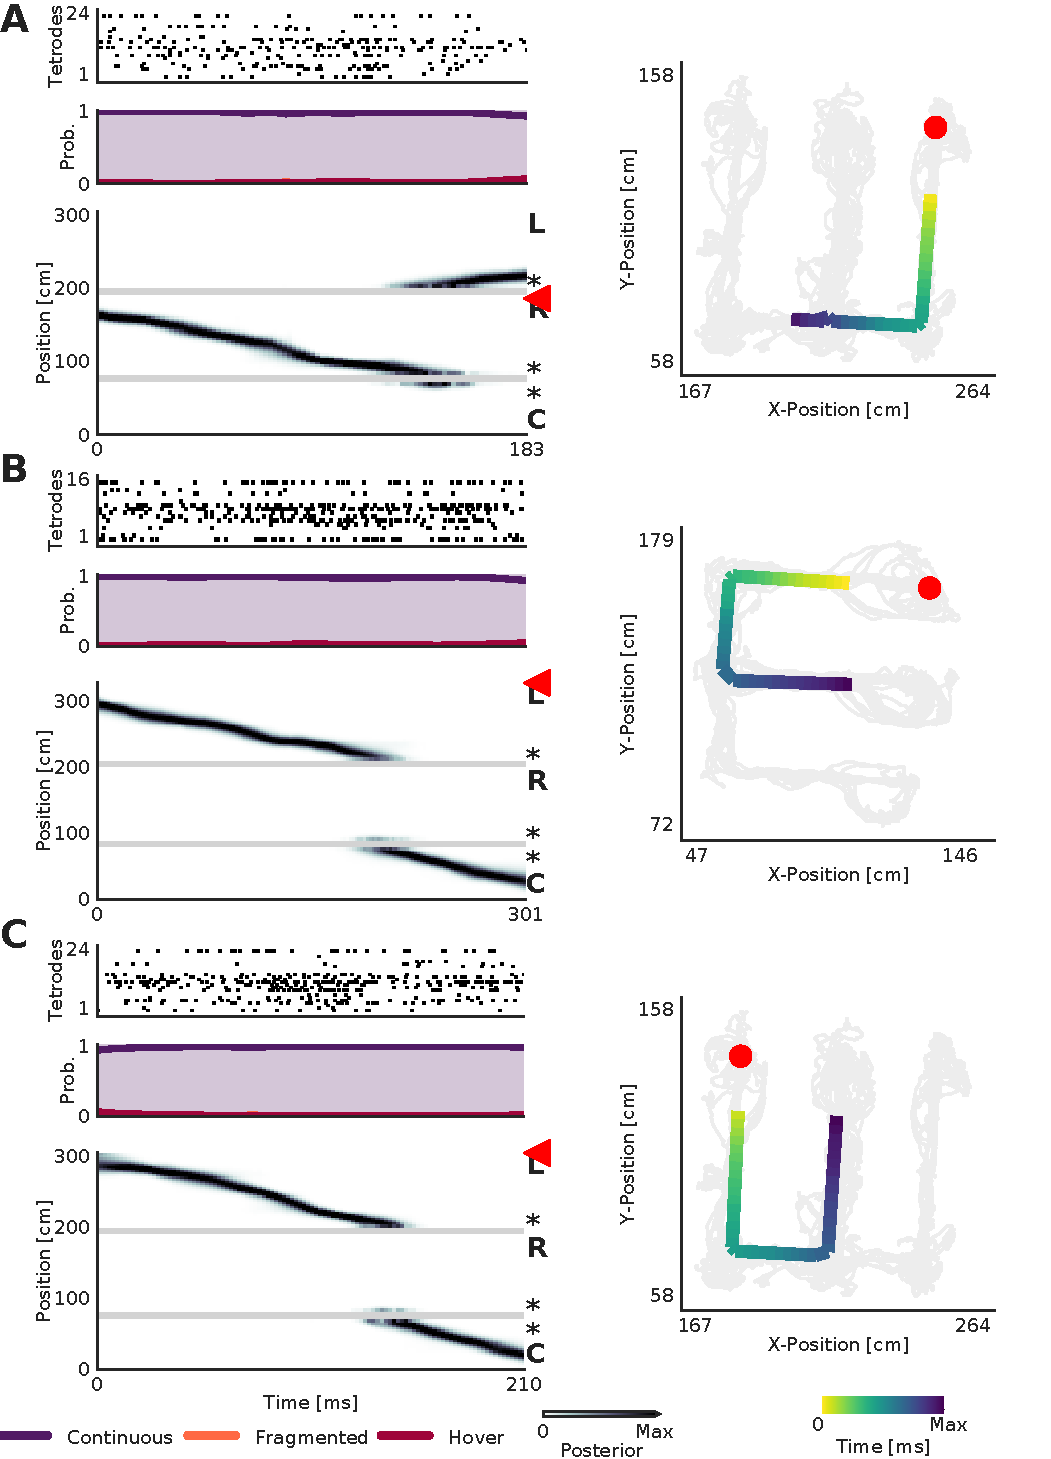
\includegraphics[width=0.80\linewidth]{figures/Figure2-supplemental2/Figure2_v2-supplemental2}
\caption{Placeholder image of Iris with a long example caption to show justification setting.}
\label{fig:Figure2-Figure supplement 2}
\end{figure*}

\begin{figure*}%[tbhp]
\centering
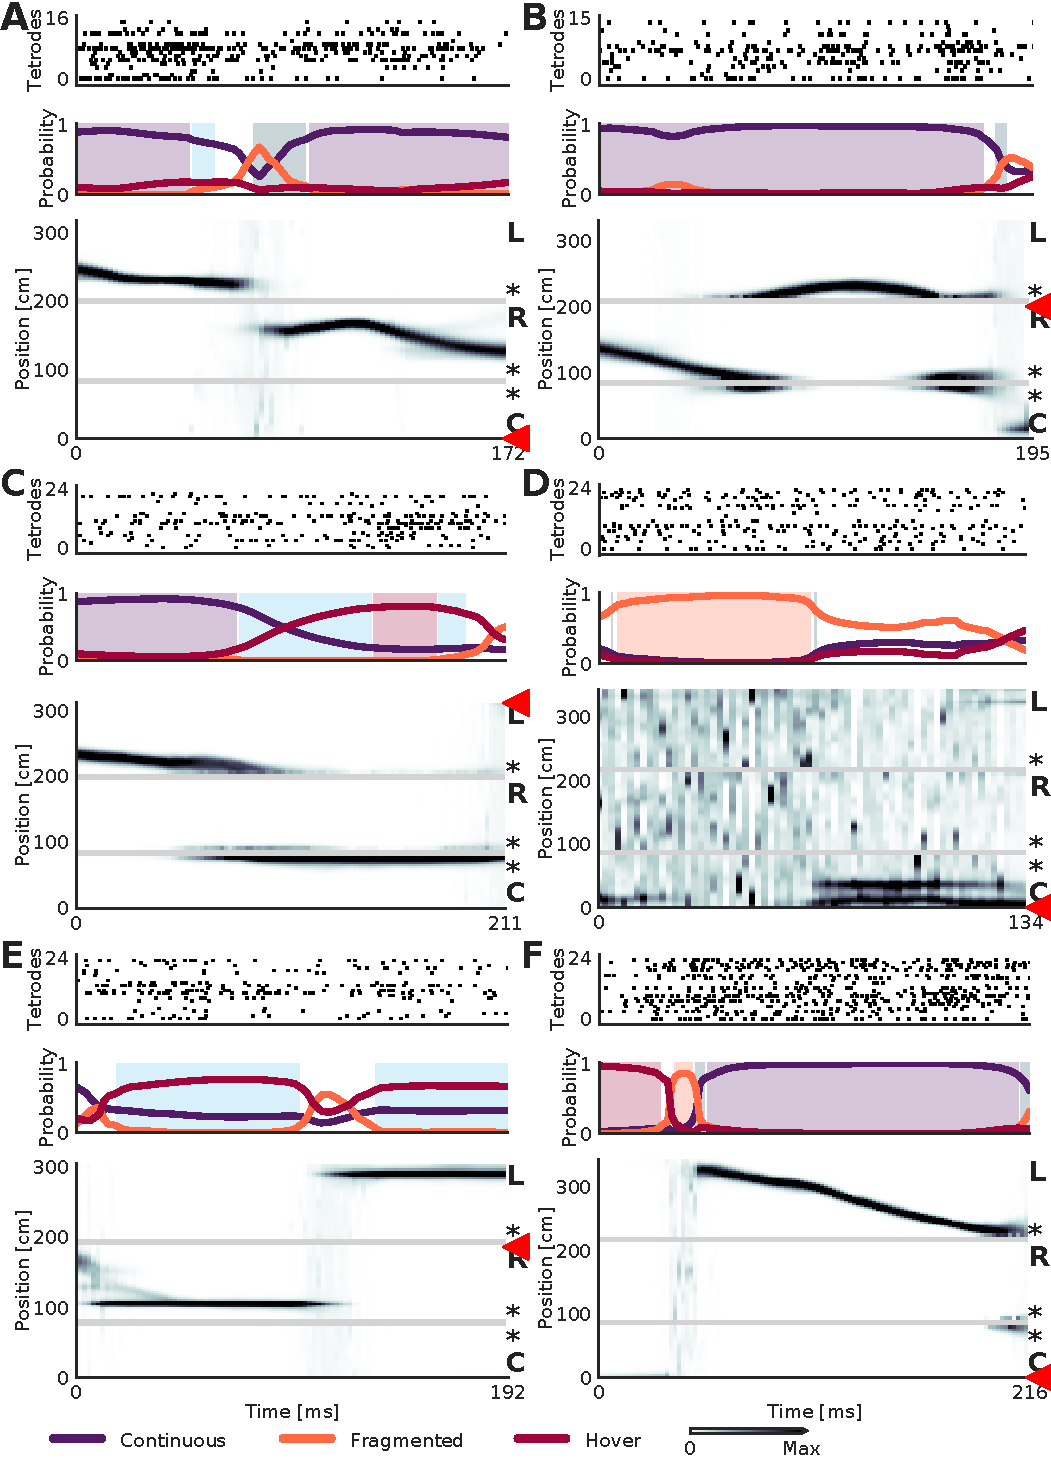
\includegraphics[width=0.80\linewidth]{figures/Figure3-supplemental1/Figure3_v2_supplemental1}
\caption{Placeholder image of Iris with a long example caption to show justification setting.}
\label{fig:Figure3-Figure supplement 1}
\end{figure*}


%TC:endignore
%the command above ignores this section for word count

\end{document}
